%!TEX program = <xelatex>
\documentclass[xetex]{beamer}
% \documentclass[draft, xetex]{beamer}

		% Iclude packages and commands used text-wide.	
%%%%%%%%%%%%%%%%%%%%%%%%%%%%%%%%%%%%%%%%%%%%%%%%%%%%%%%%%%%%%%%%%%%%%%%%%%%%%%%%%%%%%%%%%%%%%%%%%%%%%%%%%%%

\usepackage{mystyle}

		% Presentation settings.
%%%%%%%%%%%%%%%%%%%%%%%%%%%%%%%%%%%%%%%%%%%%%%%%%%%%%%%%%%%%%%%%%%%%%%%%%%%%%%%%%%%%%%%%%%%%%%%%%%%%%%%%%%%


		% Title
	\title[ETD]{MassTodon}
	\subtitle{Oprogramowanie Służące Interpretacji Widm Spektroskopu Masowego z Wykorzystaniem Techniki Dysocjacji Transferem Elektronów}

	%\beamerdefaultoverlayspecification{<+->}
	\date{9 Stycznia 2014} 
	\author[Matteo]{Mateusz Łącki}
	\institute[UW]{Uniwersytet Warszawski}
	\titlegraphic{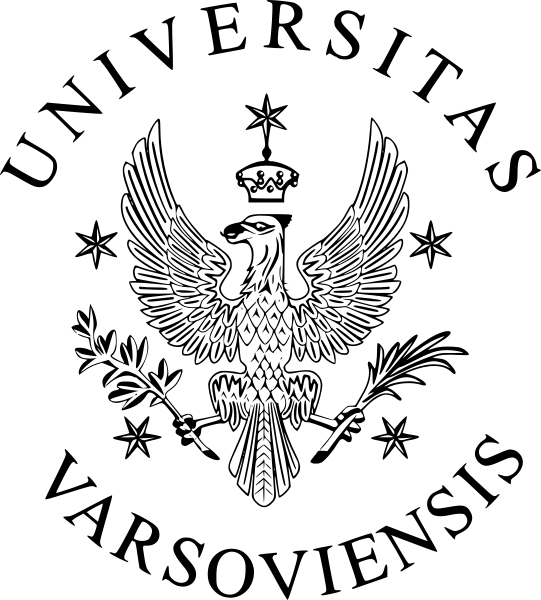
\includegraphics[scale=.10 , keepaspectratio]{./picts/eagle3.png}}
	
		% The document
%%%%%%%%%%%%%%%%%%%%%%%%%%%%%%%%%%%%%%%%%%%%%%%%%%%%%%%%%%%%%%%%%%%%%%%%%%%%%%%%%%%%%%%%%%%%%%%%%%%%%%%%%%%	

\begin{document}

	\fontspec[Numbers={OldStyle}]{Linux Libertine O}

	%%%%%%%%%%%%%%%%%%%%%%%%%%%%%%%%%%%%%%%%%%%%%%%%%%%%%%%%%%%%%%

	\begin{frame}
		\titlepage
	\end{frame}

\section[Motywacja]{Studium Przypadku}		
	%%%%%%%%%%%%%%%%%%%%%%%%%%%%%%%%%%%%%%%%%%%%%%%%%%%%%%%%%%%%%%%%%%
	\framedGraphic{Substancja P okiem Spektrometru Masowego}{./picts/inputData.png}
	%%%%%%%%%%%%%%%%%%%%%%%%%%%%%%%%%%%%%%%%%%%%%%%%%%%%%%%%%%%%%%%%%%
	\begin{frame}\frametitle{Projekt MassTodon}
		\begin{itemize}
			\item Spektrometr Masowy 
			\begin{itemize}
				\item Bada skład molekularny próbek
				\item Wynik pomiaru:
				\begin{itemize}
					\item[$\star$] $\Big\{ \frac{\text{Masa}_j}{\text{Ładunek}_j}, \text{Intensywność}_j \Big\}_j^{J}$ 
				\end{itemize}
			\end{itemize}
			\item Technologia MS/MS 
			\begin{itemize}
				\item Uszeregowienie dwu spektroskopów
				\item Filtracja molekuł o ustalonej masie do ładunku
				\item Wykorzystanie ETD
			\end{itemize}
			\item Motywacja
			\begin{itemize}
				\item Wyjaśnienie struktury spektrum posiekanego elektronami polimeru   
			\end{itemize}
		\end{itemize}
	\end{frame}

	\framedGraphic{Przydatna Analogia}{./picts/puzzles.pdf}
	%%%%%%%%%%%%%%%%%%%%%%%%%%%%%%%%%%%%%%%%%%%%%%%%%%%%%%%%%%%%%%%%%%
	\begin{frame}\frametitle{Dzisiejszy Program}
		\tableofcontents
	\end{frame}

%%%%%%%%%%%%%%%%%%%%%%%%%%%%%%%%%%%%%%%%%%%%%%%%%%%%%%%%%%%%%%%%%%		
\section[Model]{Statistical Modelling}
%%%%%%%%%%%%%%%%%%%%%%%%%%%%%%%%%%%%%%%%%%%%%%%%%%%%%%%%%%%%%%%%%%
	\begin{frame}\frametitle{{\color{gray}Produkt} Model{\color{gray}ów} Wielomianowy{\color{gray}ch}}
		    
		\begin{itemize}
			\item Czemu służy?
			\begin{itemize}
				\item Rozkład Liczby Dodatkowych Neutronów
				\item Rozkład Masy Związku Chemicznego
				\item Odchył od obserwowanej masy monoizotopowej
			\end{itemize}
		\end{itemize}

		\begin{center}
			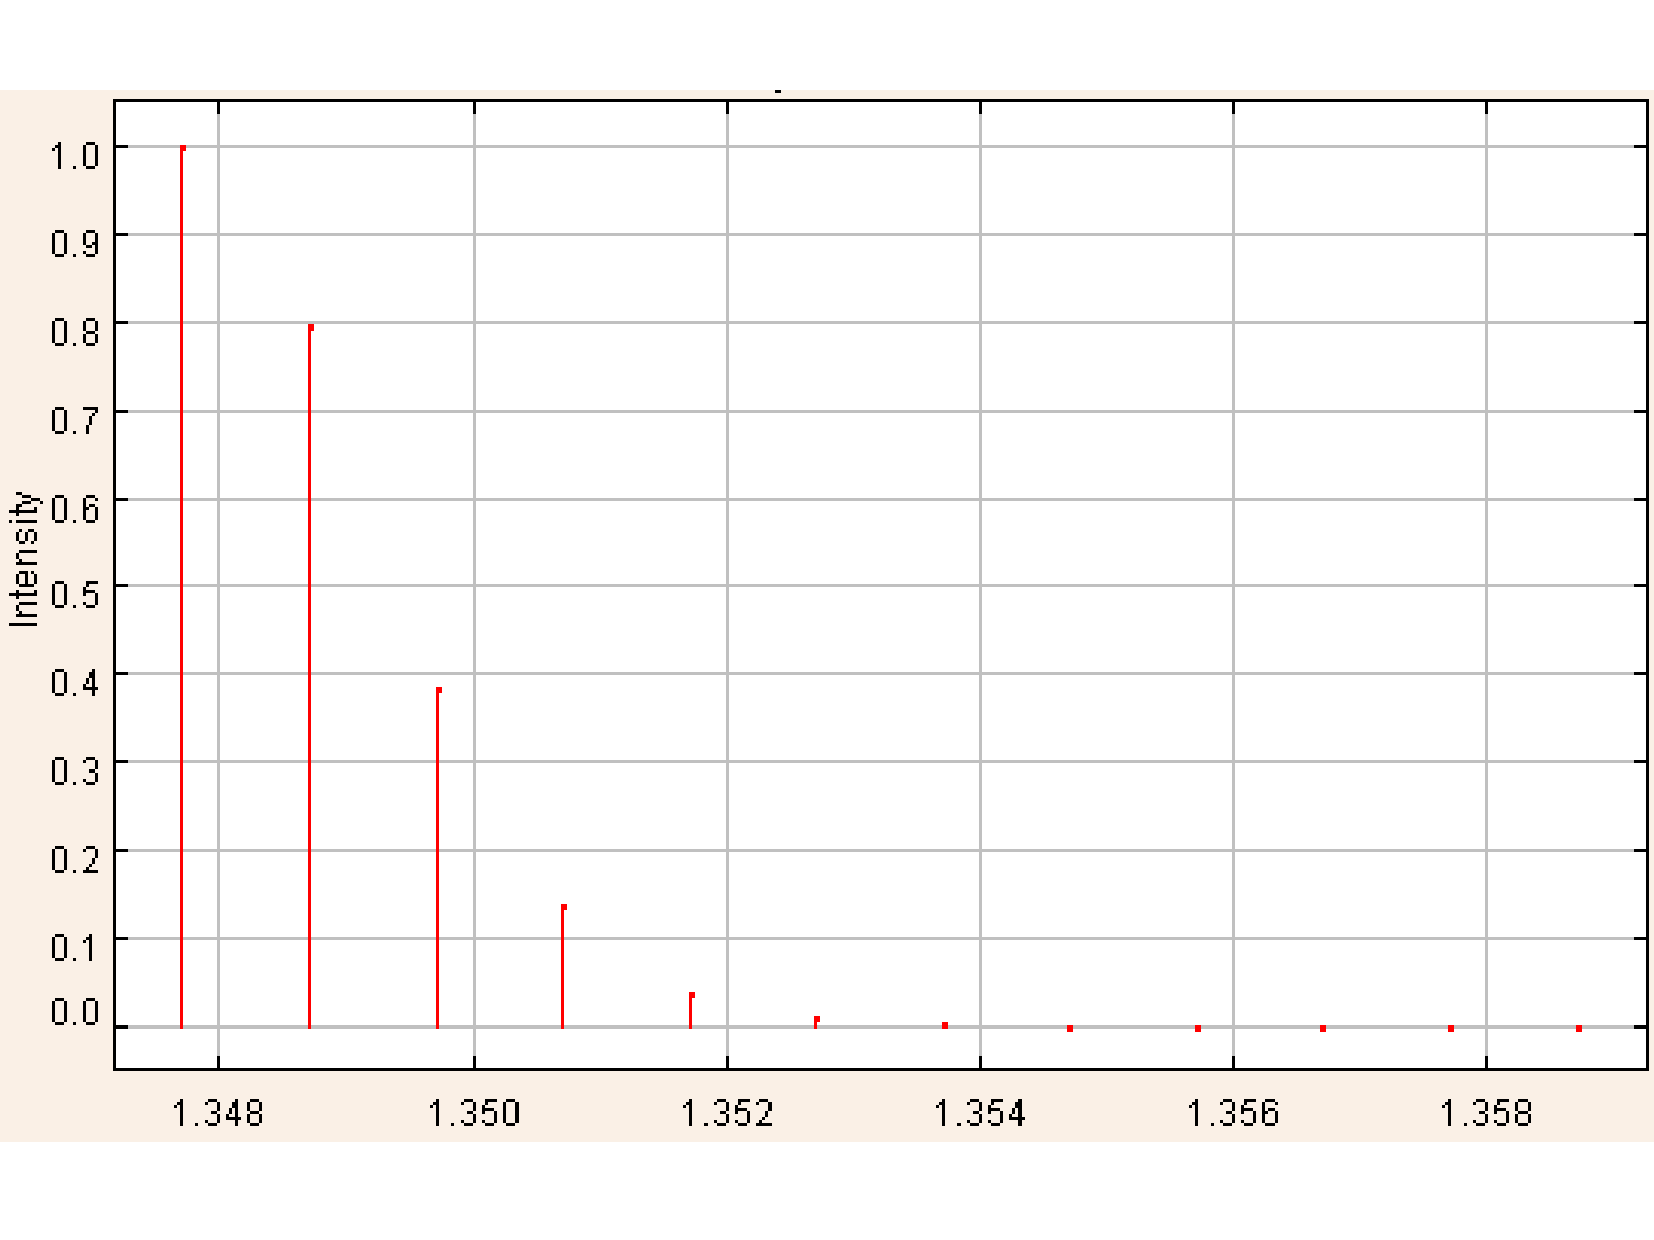
\includegraphics[height=.5\textheight, keepaspectratio]{./picts/realMassDistribution.pdf}
		\end{center}
	\end{frame}	

	%%%%%%%%%%%%%%%%%%%%%%%%%%%%%%%%%%%%%%%%%%%%%%%%%%%%%%%%%%%%%%%%%%
	\begin{frame}\frametitle{Model Wielomianowy}

		\begin{itemize}
			\item Rozkład Liczby Dodatkowych Neutronów w {\it przyrodzie}
			\begin{itemize}
				\item $\prob( \cem{^{16}O} ) = 99.757$
				\item $\prob( \cem{^{17}O} ) = 0.038$
				\item $\prob( \cem{^{18}O} ) = 0.205$
				\item[źródło:] \textcolor{adriatico}{I}nternational \textcolor{adriatico}{U}nion of \textcolor{adriatico}{P}ure and \textcolor{adriatico}{A}pplied \textcolor{adriatico}{C}hemistry 1997 
			\end{itemize}
			\item Molekuła = \molecule
			\item Założenia
			\begin{itemize}
				\item 	Dużo niezależności: izotop danego atomu \molecule (np. \ce{C}) nie zależy od izotopów pozostałych atomów
				\begin{itemize}
					\item[np.]  molekuła trój-atomowa wody
				\end{itemize}				  
				$$\prob( \cem{^{1}H ^{2}H ^{17}O} ) = 
					\prob( \cem{^{1}H} ) \times \prob( \cem{^{2}H} ) \times \prob( \cem{ ^{17}O} ) $$
				\item 	Nie rozróżniamy izomerów
				$$ \cem{^{13}C ^{17}O ^{17}O} \simeq \cem{^{17}O ^{13}C ^{17}O} \simeq \cem{ ^{17}O ^{17}O ^{13}C }$$	
			\end{itemize}
		\end{itemize}

	\end{frame}

	%%%%%%%%%%%%%%%%%%%%%%%%%%%%%%%%%%%%%%%%%%%%%%%%%%%%%%%%%%%%%%%%%%
	\begin{frame}\frametitle{{\color{gray}Produkt} Model{\color{gray}ów} Wielomianowy{\color{gray}ch}}
			
		\begin{itemize}
			\item Związek Chemiczny = lista zbiorów atomów 

		\end{itemize}
		\begin{center}
			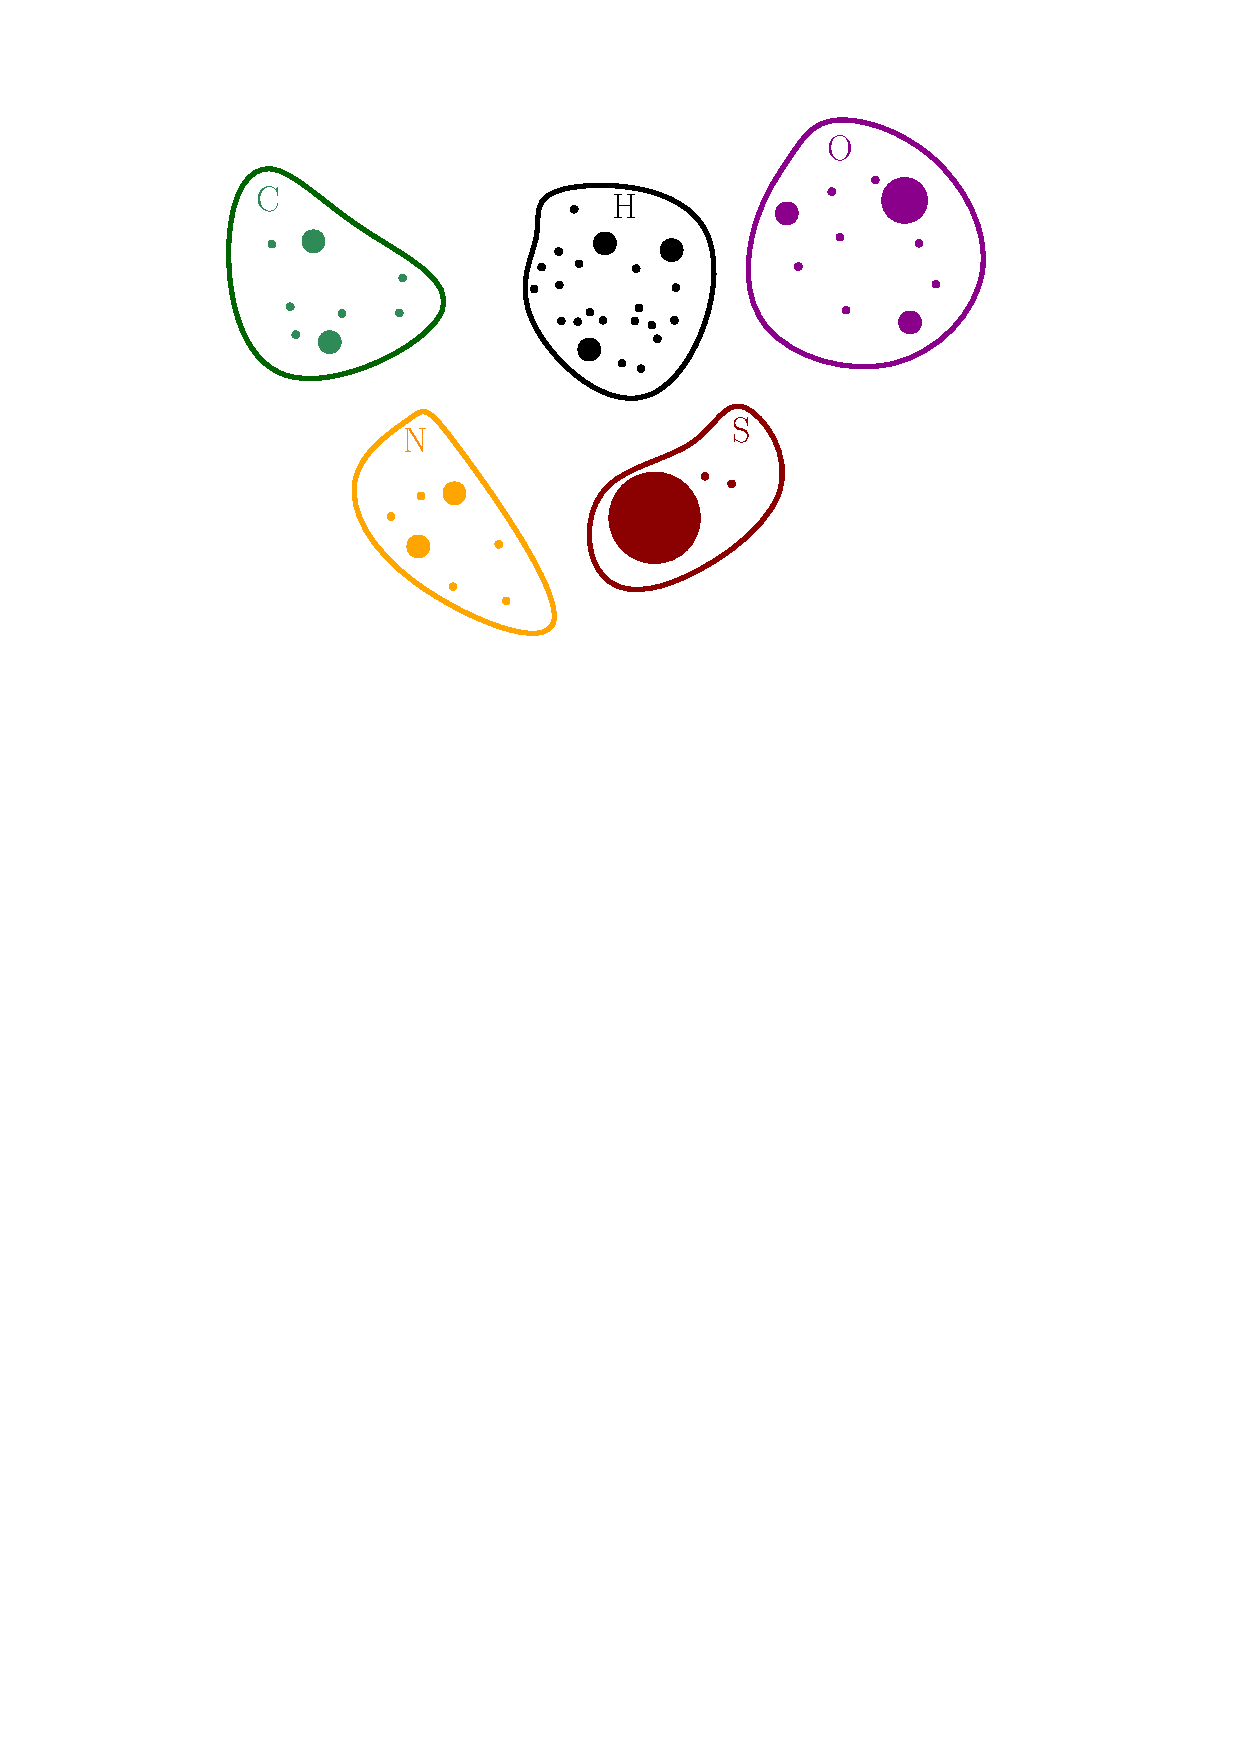
\includegraphics[height=.4\textheight, keepaspectratio]{./picts/molecule.pdf}
		\end{center}

		$$ \prob( 
			\underbrace{\cem{c_{12}} \cem{^{12}C},\, \cem{c_{13}} \cem{^{13}C}}_{\cem{c_{12}}+ \cem{c_{13}} = \cem{c}},\,
			\underbrace{\cem{h_1} \cem{^{1}H},\,\cem{h_2} \cem{^{2}H}}_{\cem{h_1} + \cem{h_2} = \cem{h}}, 
			\,\dots,\, 
			\cem{s_{36}} \cem{^{36}S} ) 
			= 
			$$

		$$ 	{\cem{c} \choose \cem{c_{12}},\cem{c_{13}} }
			\prob(\cem{^{12}C})^{\cem{c_{12}}} \prob(\cem{^{13}C})^{\cem{c_{13}}} 
			{\cem{h} \choose \cem{h_{1}},\cem{h_{2}} }
			\prob(\cem{^{1}H})^{\cem{h_1}} \prob(\cem{^{2}H})^{\cem{h_2}}
			\dots $$	

	\end{frame}


	%%%%%%%%%%%%%%%%%%%%%%%%%%%%%%%%%%%%%%%%%%%%%%%%%%%%%%%%%%%%%%%%%%
	\begin{frame}\frametitle{{\color{gray}Produkt} Model{\color{gray}ów} Wielomianowy{\color{gray}ch} a Masa Molekuł}
		
		\begin{itemize}
			\item $m_W$ masa molekuły $W = (\cem{c_{12}}, \cem{c_{13}}, \dots, \cem{s_{36}})$ 
			\begin{itemize}
				\item[$\star$] $m_W = \cem{c_{12}} m_\cem{^{12}C} + \dots + \cem{s_{36}} m_\cem{^{36}S}$

				\item[$\star$] $\prob( \text{Masa Molekuły} = m ) = 
					\sum_{W: m_W = m} \prob(
						\cem{c_{12}} \cem{^{12}C}, 
						\dots, 
						\cem{s_{36}} \cem{^{36}S} )$
				\item[s.t.] $m_W = \cem{c_{12}} m_\cem{^{12}C} + \dots + \cem{s_{36}} m_\cem{^{36}S}$
				\item[:)] Wzór $W \rightarrow$ miara $p_W \rightarrow \rightarrow$
				\item[:(] Ilość pików rośnie.  
			\end{itemize}
			\item Fakt
			\begin{itemize}
				\item 	Dodatkowe neutrony zmieniają masę pierwiastków różnorako   
				\item  	Różnice są możliwe do zaobserwowania w spektroskopie
			\end{itemize}
			\item[$\bigstar$] Algorytm BRAIN zaniedbuje powyższą właściwość materii
		\end{itemize}



	\end{frame}

	%%%%%%%%%%%%%%%%%%%%%%%%%%%%%%%%%%%%%%%%%%%%%%%%%%%%%%%%%%%%%%%%%%
	\begin{frame}\frametitle{Wizualizacja Modelu Wielomianowego}

		\begin{itemize}
			\item Oprogramowanie BRAIN - Piotr Dittwald$^\text{\textregistered}$
			\item Założenie: 
			\begin{itemize}
				\item[$\star$] Neutrony mają masę 1 Daltona dla wszystkich pierwiastków.
			\end{itemize}
		\end{itemize}

		\begin{columns}
			\begin{column}[t]{.5\textwidth}
				\begin{center}
					Etanol 
					\ce{C_2 H_5 OH}
					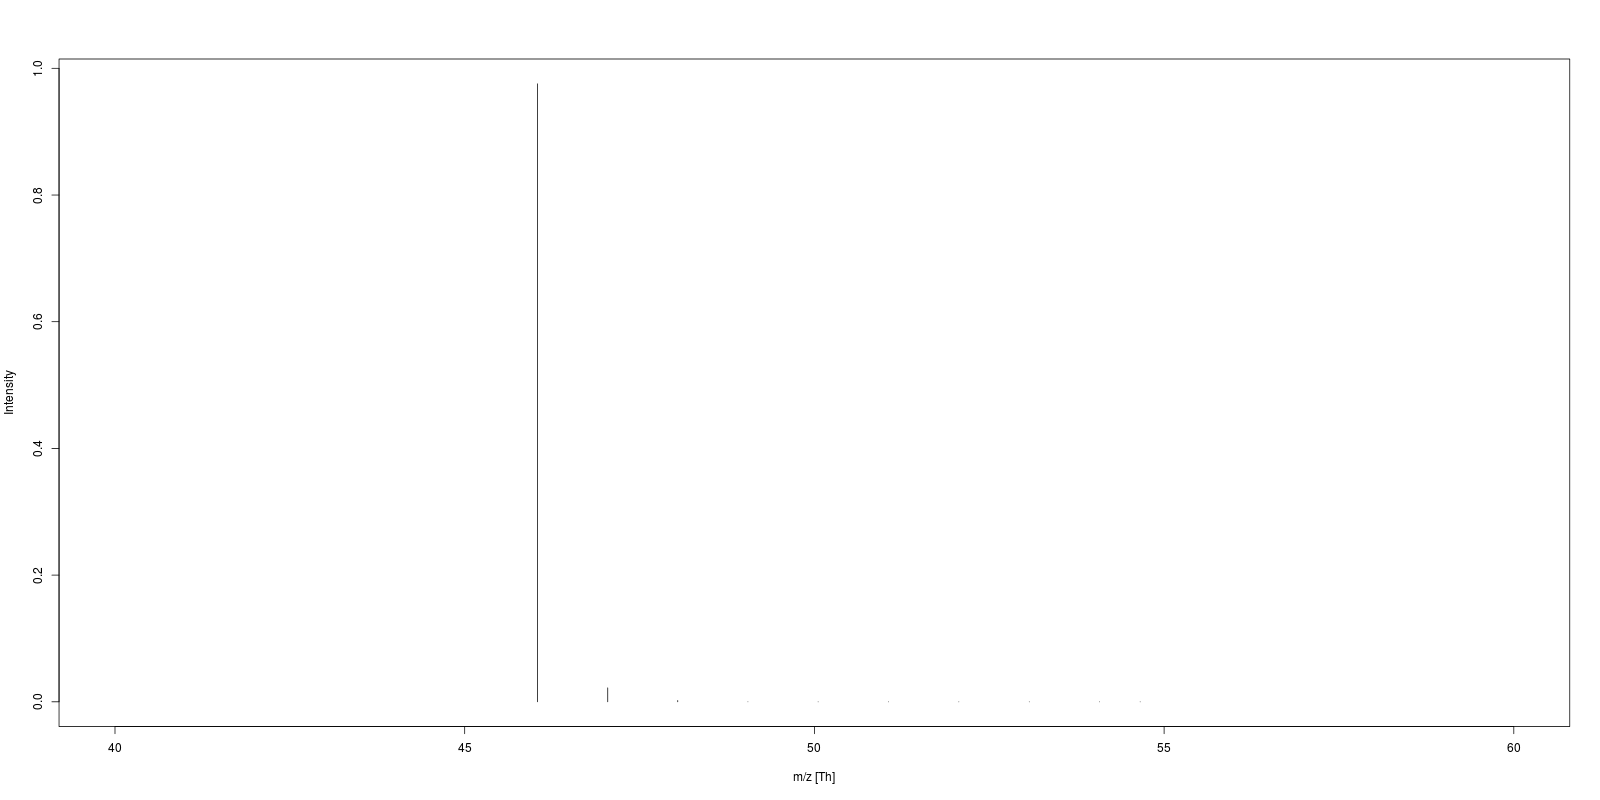
\includegraphics[height=.3\textheight, keepaspectratio]{./picts/ethanol.png}
				\end{center}
			\end{column}
			\begin{column}[t]{.5\textwidth}
				\begin{center}
					Angiotensyna II
					\ce{C_{50} H_{71} N_{13} O_{12}}
					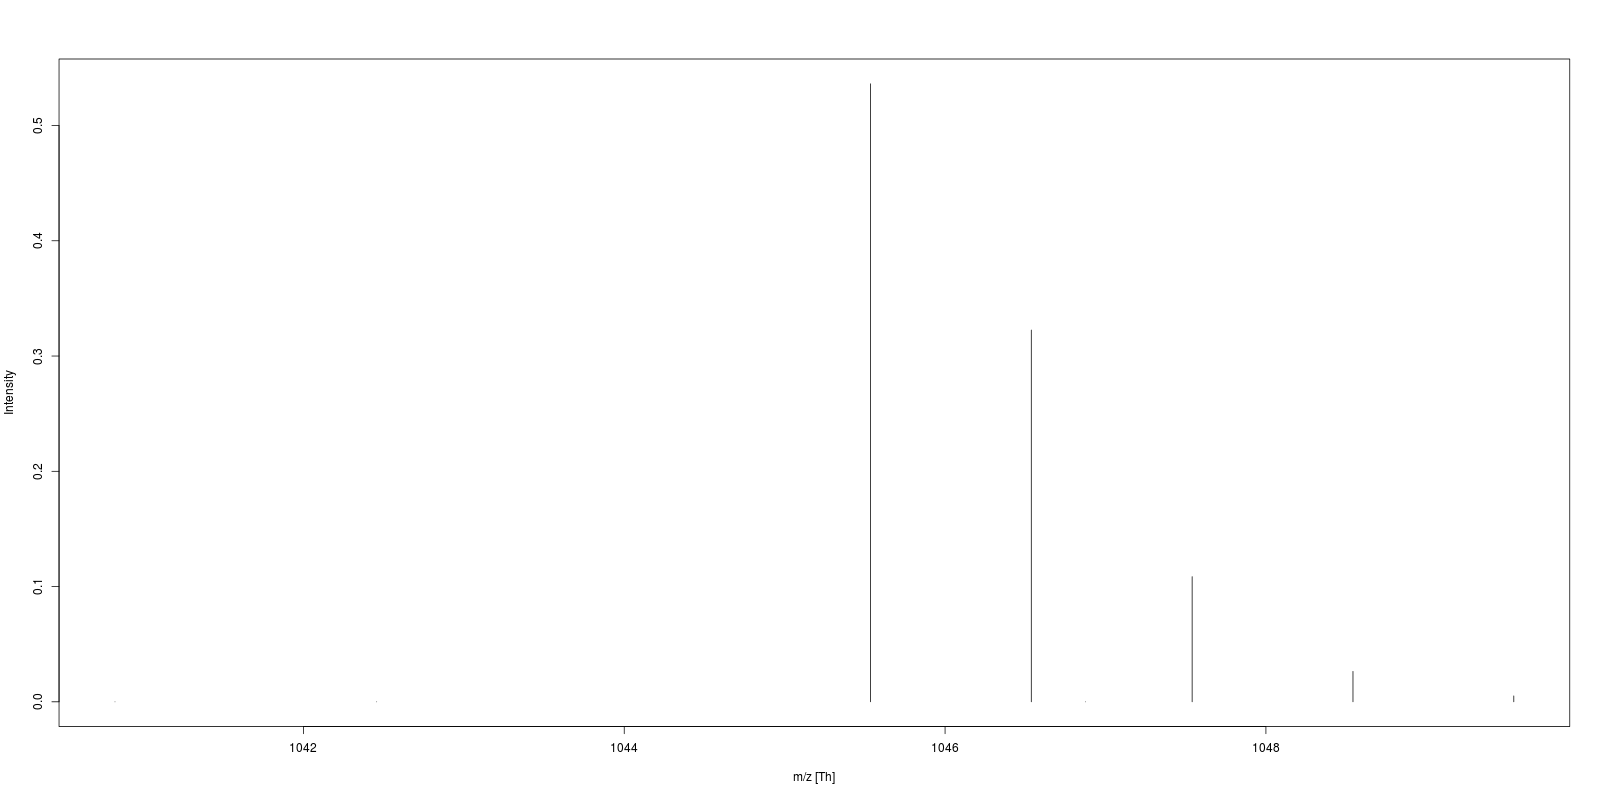
\includegraphics[height=.3\textheight, keepaspectratio]{./picts/angiotensine.png}		
				\end{center}
			\end{column}
		\end{columns}	

		\begin{itemize}
			\item Hola hola! Spekrum z początkowego slajdu było wielomodalne!
			\begin{itemize}
				\item fragmentacja (ETD)
				\item szafowanie ładunkami (ETD, ETnoD, PTR)
			\end{itemize}
		\end{itemize}
	\end{frame}	

	\framedGraphic{Substancja P okiem Spektrometru Masowego}{./picts/inputData.png}

	%%%%%%%%%%%%%%%%%%%%%%%%%%%%%%%%%%%%%%%%%%%%%%%%%%%%%%%%%%%%%%%%%%
	\begin{frame}\frametitle{Polimery jako sekwencje aminokwasów}
		\begin{center}
			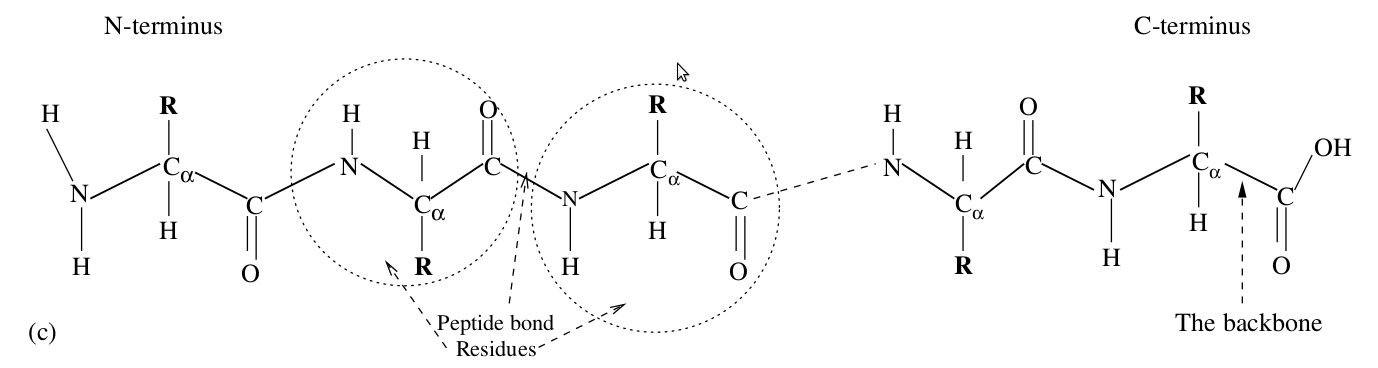
\includegraphics[height=.35\textheight, keepaspectratio]{./picts/aminos.png}
		\end{center}		

		\begin{itemize}
			\item Dodatkowa struktura pomiędzy wzorem sumarycznym a poszczególnymi pierwiastkami
			\begin{itemize}
				\item[] \molecule = $A_1 A_2 \dots A_k$
				\item[] $A_i \in \{ \text{
				Alanina, Cysteina, Kwas Asparaginowy, Kwas Glutaminowy, \dots
				} \}$
			\end{itemize}
		\end{itemize}

	\end{frame}

	\framedGraphic{Dodatkowa struktura - sekwencje aminokwasów}{./picts/moleculeSubdivided.pdf}

	%%%%%%%%%%%%%%%%%%%%%%%%%%%%%%%%%%%%%%%%%%%%%%%%%%%%%%%%%%%%%%%%%%	
	\begin{frame}\frametitle{Electron Transfer Disociation}
		\begin{itemize}
			\item Wynik: losowe cięcię białka na dwa podsłowa 
			$$ A_1 A_2 \dots A_k \rightarrow 
				\underbrace{A_1 \dots A_L}_\text{$C$-fragment}  \oplus \underbrace{A_{L+1} \dots A_k}_\text{$Z$-fragment}$$
			\item $L$ = numer przeciętego wiązania peptydowego (od N do C) 					
		\end{itemize}

		\begin{columns}
			\begin{column}[t]{.5\textwidth}
				\begin{itemize}
					\item Założenia
				\begin{itemize}
					\item $L$ nie zależy od składu izotopowego
					$$ \prob( A_1 \dots A_L = a_1 \dots a_L | L=l ) = 
					$$
					$$ \prob( A_1 \dots A_l = a_1 \dots a_l)$$
				\end{itemize}
					\item Drobna komplikacja: dodatkowe wiązania peptydowe na $A_1$ - wprowadzamy stan $L=0$ 
				\end{itemize}
			\end{column}
			\begin{column}[t]{.5\textwidth}
				\begin{center}
					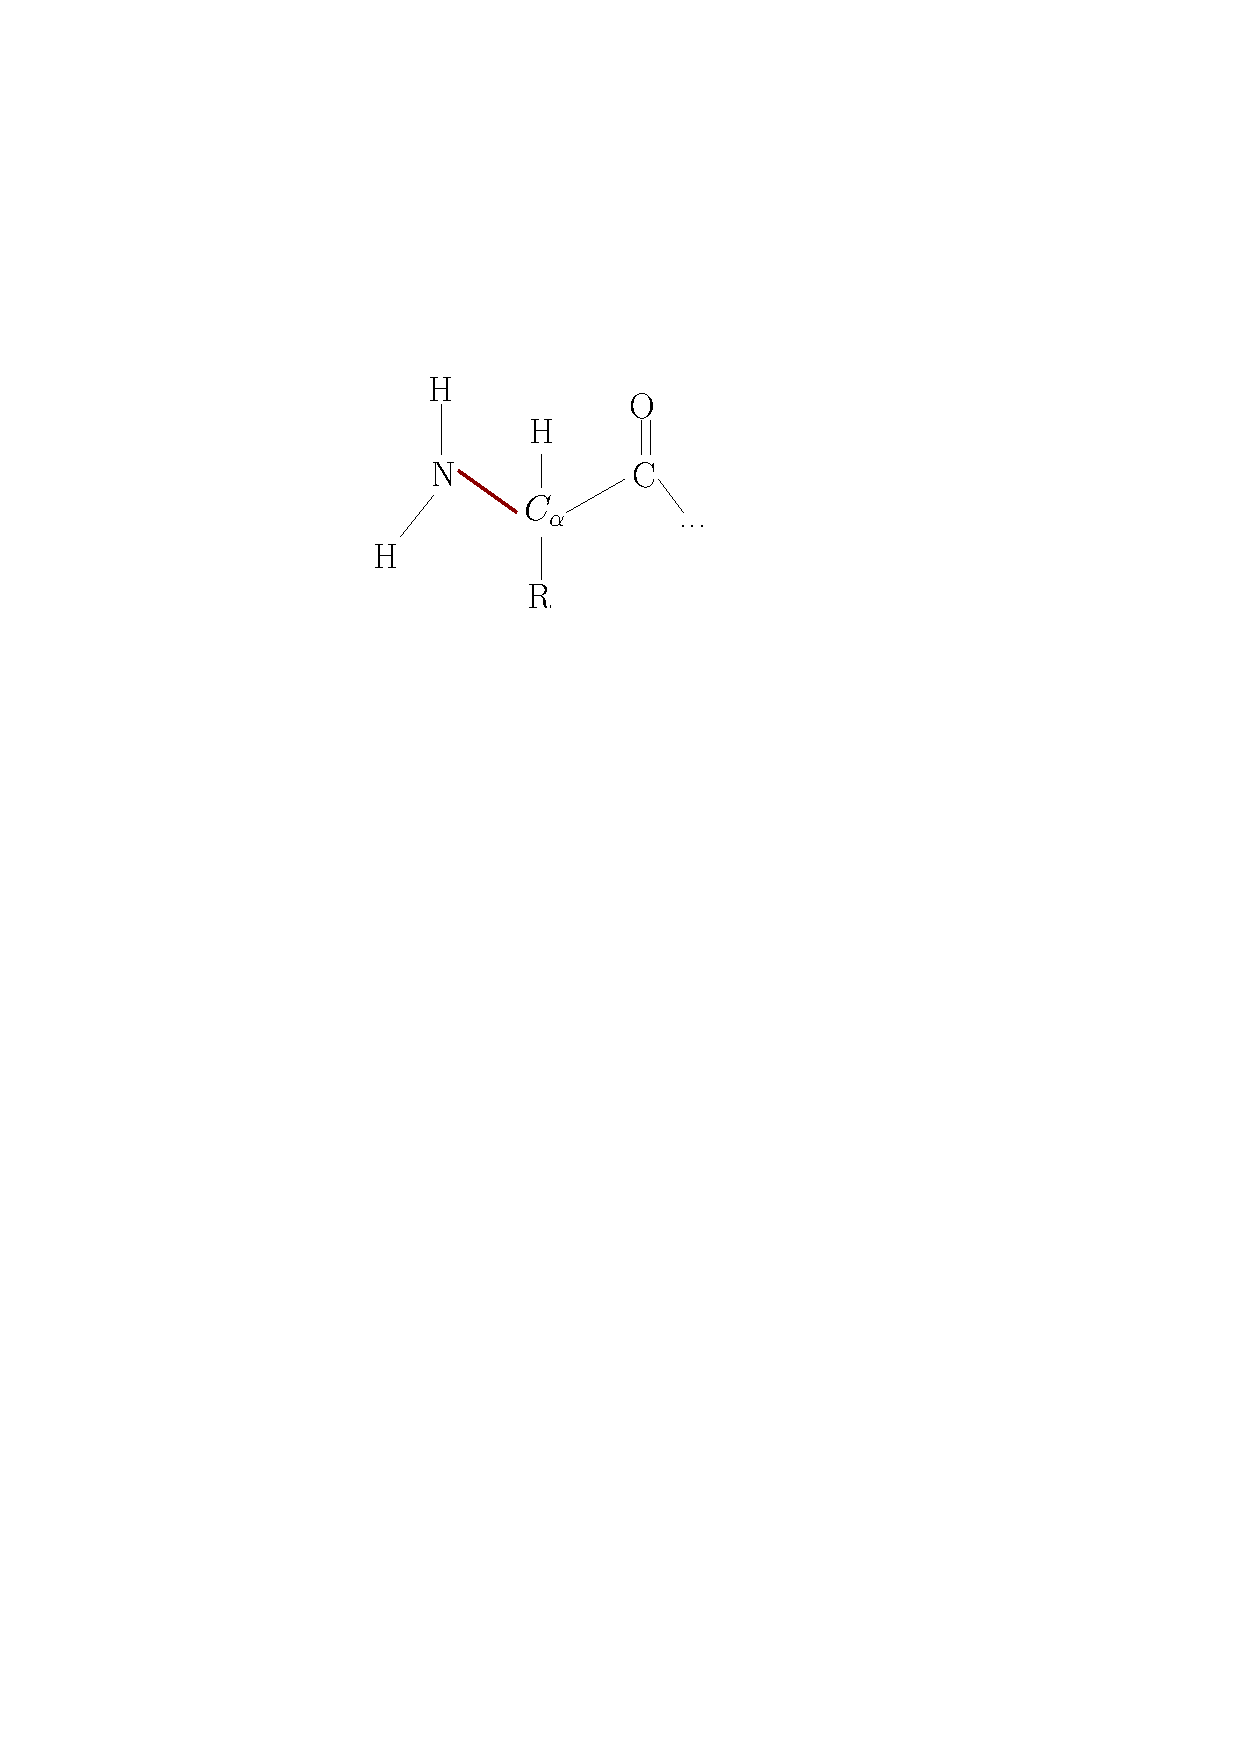
\includegraphics[height=.30\textheight, keepaspectratio]{./picts/aminoAcid.pdf}
				\end{center}
			\end{column}
		\end{columns}
	\end{frame}

	%%%%%%%%%%%%%%%%%%%%%%%%%%%%%%%%%%%%%%%%%%%%%%%%%%%%%%%%%%%%%%%%%%
	\begin{frame}\frametitle{Możliwe reakcje okiem zaprzyjaźnionego chemika Friderika}
		\begin{itemize}
			\item[] Hipoteza:
			\begin{itemize}
				\item[$\star$] Spektrum Empiryczne = Wynik Kilku Reakcji
			\end{itemize}
			\item ETD
			\begin{center}
				\ce{[M $+$ n H]^{n+} + A^{.$-$} -> [C $+$ x H]^{x+} + [Z $+$ (n$-$x)H]^{(n$-$x$-1$).} + A}
			\end{center}
			\item PTR
			\begin{center}
				\ce{[M $+$ n H]^{n+} + A^{.$-$} -> [M $+$ (n$-1$ ) H]^{(n$-1$)+} + AH}
			\end{center}			
			\item ETnoD
			\begin{center}
				\ce{[M $+$ n H]^{n+} + A^{.$-$} -> [M $+$ n H]^{(n$-1$)+.} + A}
			\end{center}			
			\item To nie jest poprawny zapis reguł
			\begin{itemize}
			 	\item[e.g.] Błędy w konkatenacjach reakcji: $ETD \rightarrow PTR \rightarrow PTR \rightarrow ETnoD$  
			\end{itemize} 			
		\end{itemize}
	\end{frame}

	%%%%%%%%%%%%%%%%%%%%%%%%%%%%%%%%%%%%%%%%%%%%%%%%%%%%%%%%%%%%%%%%%%
	\begin{frame}\frametitle{Poprawne Zasady}
		
		\begin{itemize}
			\item Dodatowy opis molekuły o wzorze \molecule - para $(p,q)$
			\begin{itemize}
				\item $p$ - {\it protonizacja}
				\begin{itemize}
					\item liczba dodatkowych protonów bez sparowanych elektronów
					\item to ładunek molekuły
					\item to coś waży
				\end{itemize}
				\item $q$ - {\it zneutralizowana protonizacja}
				\begin{itemize}
					\item liczba dodatkowych protonów ze sparowanymi elektronami
					\item to coś waży ale jest elektycznie obojętne
				\end{itemize}				
			\end{itemize}
			\item Wsad algorytmu: $(A_1 A_2 \dots A_k, p , q)$ 
		\end{itemize}
	\end{frame}

	%%%%%%%%%%%%%%%%%%%%%%%%%%%%%%%%%%%%%%%%%%%%%%%%%%%%%%%%%%%%%%%%%%
	\begin{frame}\frametitle{Możliwe Reakcje: o potrzebie rachunkowości w przyrodzie}
		
		\begin{itemize}
			\item Wsad: $(A_1 A_2 \dots A_k,\, p ,\, q)$ 
			\item Reakcje Cząstkowe
				\begin{itemize}
				\item[$\clubsuit$] ETD
				\begin{itemize}
					\item[$\rightarrow$] $ (A_1 \dots A_L,\, p_1,\, q_1) $
					\item[$\rightarrow$] $ (A_{L+1} \dots A_k,\, p_2,\, q_2) $
					\item[że]$p_1 + p_2 = p -1$ oraz $q_1 + q_2 = q$ i $q_2 \geq 0$
				\end{itemize}
				\item[$\diamondsuit$] PTR 
				\begin{itemize}
					\item[$\rightarrow$] $ (A_1 \dots A_k,\, p-1,\, q)$ 
				\end{itemize}
				\item[$\heartsuit$] ETnoD 
				\begin{itemize}
					\item[$\rightarrow$] $ (A_1 \dots A_k,\, p-1,\, q+1)$ 
				\end{itemize}
				\item[$\spadesuit$] \emph{HTR}
				\begin{itemize}
					\item[$\rightarrow$] $ (A_1 \dots A_L,\, p_1,\, q_1)$,
					\item[$\rightarrow$] $ (A_{L+1} \dots A_k,\, p_2,\, q_2)$,
					\item[że] $p_1 + p_2 = p$ oraz $q_1 + q_2 = q + 1$ i $q_2 \geq 1$
				\end{itemize}	
			\end{itemize}
		\end{itemize}
	\end{frame}

	%%%%%%%%%%%%%%%%%%%%%%%%%%%%%%%%%%%%%%%%%%%%%%%%%%%%%%%%%%%%%%%%%%
	\begin{frame}\frametitle{Algorytm - generowanie wzorów chemicznych}

		\begin{itemize}
			\item $S = \Big[M = A_1 \dots A_k,\, p = \text{Maksymalne Naładowanie}, q = 0\Big]$

			\begin{itemize}
			
				\item Reakcje Cząstkowe $ = $ 
					$$ = \{ 
					\mathfrak{Id},\,
					\clubsuit^C_{L , p_1, q_1},\,
					\clubsuit^Z_{L,p_2, q_2},\, 
					\diamondsuit,\, 
					\heartsuit,\, 
					\spadesuit^C_{L,\tilde{p}_1, \tilde{q}_1},\, 
					\spadesuit^Z_{L,\tilde{p}_2, \tilde{q}_2} \} $$
				\item  
					$$ \text{Reakcje}= \{ r_1 r_2 \dots r_k : r_i \text{ to reakcja cząstkowa i jest OK} \} $$
				\item[np.] $\Big(\clubsuit^C_{L, 2,1} \heartsuit$ $\heartsuit \diamondsuit\Big)$ może być OK jeśli 

				\begin{itemize}
					\item $S$ ma wystarczająco ładunków
					\item $M$ jest wystarczająco długa
					\item $q$ protonów zostało {\it zneutralizowanych} przed ET 
				\end{itemize}
			
			\end{itemize}

			\item 	Wynik pełny: lista trójek $\Biggl\{[W, p_W, q_W]\Biggl\}_{W \in \text{Reacje}}$  
		\end{itemize}
	\end{frame}

	%%%%%%%%%%%%%%%%%%%%%%%%%%%%%%%%%%%%%%%%%%%%%%%%%%%%%%%%%%%%%%%%%%
	% \item  	Spektrum empriczne, $y = \Big\{ ( \frac{m_j}{z_j}, I_j) \Big\}_{j = 1}^{J}$
	
	\begin{frame}\frametitle{Rozkłady indukowane przez reakcje}
		\begin{itemize}
			\item Rozkład na osi $\frac{m}{z}$: 
	
			\begin{itemize}
				\item 	Algorytm dostarcza trójek $R = [ W, p, q]$ 
				\item 	$W \rightarrow$ Model Wielomianowy $\rightarrow$ Rozkład masy $m_W \rightarrow$ 
					$$ \prob\Big(\frac{m_R}{z_R}\Big)  = \prob\Big(\frac{m_W + p + q}{p}\Big) = p_W (m_W)$$
			\end{itemize}
		\end{itemize}
	\end{frame}

	\framedPlainGraphic{width=\textwidth}{./picts/spectraShifts.png}

	%%%%%%%%%%%%%%%%%%%%%%%%%%%%%%%%%%%%%%%%%%%%%%%%%%%%%%%%%%%%%%%%%%
	\begin{frame}\frametitle{Konsekwencje zaniedbania czasu}	
		\begin{itemize}
			\item Niektóre reakcje dają te same wyniki!
				$$\heartsuit \diamondsuit = \diamondsuit \heartsuit$$
			\begin{itemize}
				\item Model abstrahuje od czasu przeprowadznia reakcji
				\item Rozróżnialne Reakcje $\subset$ Reakcje
				\item Reakcje $:=$ Klasy Równoważności w zbiorze Reakcji 
			\end{itemize}
		\end{itemize}
	\end{frame}


	%%%%%%%%%%%%%%%%%%%%%%%%%%%%%%%%%%%%%%%%%%%%%%%%%%%%%%%%%%%%%%%%%%
	\begin{frame}\frametitle{Doprecyzowanie Hipotezy Badawczej} 
		\begin{itemize}
			\item 	Spektrum Empiryczne: $y = \Big\{ (\frac{m_j}{z_j}, I_j) \Big\}_{j = 1}^{J}$
			\item[] Hipoteza
			\begin{itemize}
				\item[$\star$] $I_j = \sum_{R \in \text{Reakcje}} \alpha_R \prob(\frac{m_R}{z_R}) + \text{Błąd}$
				\item[że] $\alpha_R \geq 0,$ 
				\item[i] $\sum_R \alpha_R \leq 1$
			\end{itemize}
			\item[]
			\item 	Potrzeba oprogramowania które
			\begin{itemize}
				\item 	znajduje zbiór nierozróżnialnych reakcji $R$
				\item 	estymuje $\alpha_R$ minimalizując błąd
			\end{itemize}
		\end{itemize}
	\end{frame}

%%%%%%%%%%%%%%%%%%%%%%%%%%%%%%%%%%%%%%%%%%%%%%%%%%%%%%%%%%%%%%%%%%
\section[Dopasowanie]{Procedury Dopasowujące}	

	\framedPlainGraphic{width=\textwidth}{./picts/spectraShiftsAndWeights.png}
%%%%%%%%%%%%%%%%%%%%%%%%%%%%%%%%%%%%%%%%%%%%%%%%%%%%%%%%%%%%%%%%%%

	\begin{frame}\frametitle{massTodon}
		\begin{itemize}
			\item 	Prototyp istnieje
			\begin{figure}
				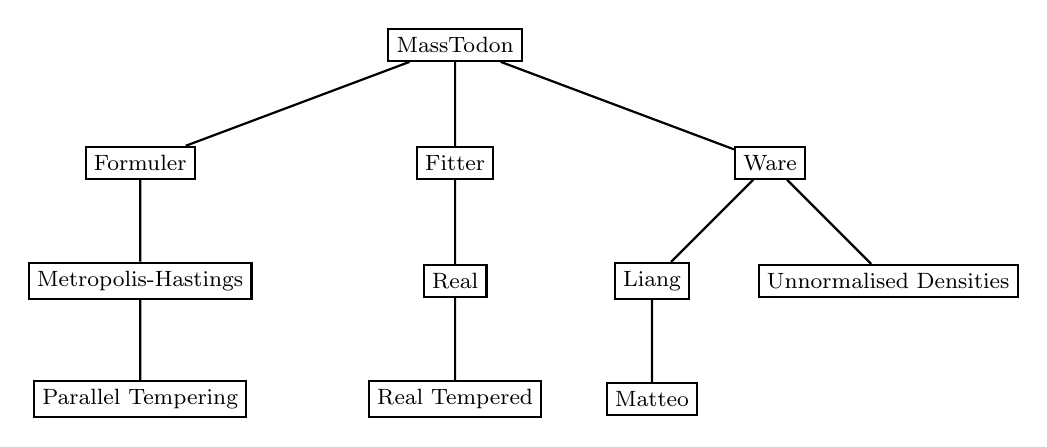
\begin{tikzpicture}
					[-,thick,%
					  every node/.style={shape=rectangle,inner sep=3pt,draw,thick}]
					\footnotesize
					\node {MassTodon}
					  [sibling distance=4cm]
					  child {node {Formuler}
					  	child {node {Metropolis-Hastings}
					  		child {node {Parallel Tempering}	
					  		}
					  	}	
					  }
					  child {node {Fitter}
					    child {node {Real}
					    	child {node {Real Tempered}
					    	}
					    }
					  }
					  child {node {Ware}
					    [sibling distance=3cm]
					    child {node {Liang}
					    	child {node {Matteo}}
					    }
					    child {node {Unnormalised Densities}}
					  };
				\end{tikzpicture}
				\caption{Current operational entity-relations diagram.}\label{objectStructure}
			\end{figure}
			Stupid fitting procedure: does not use BRAIN
		\end{itemize}
	\end{frame}

	%%%%%%%%%%%%%%%%%%%%%%%%%%%%%%%%%%%%%%%%%%%%%%%%%%%%%%%%%%%%%%%%%%
	\begin{frame}\frametitle{Kernelizacja}

		\begin{itemize}
			\item $y = \Big\{ (\frac{m_j}{z_j}, I_j) \Big\}_{j = 1}^{J}$
			\item Ale może lepiej wygładzić wszystko?
				$$ y(z) = \sum_{j=1}^J I_j \times y_j (z)$$
			\begin{itemize}
			 	\item[s.t.]$y_j (z) = \frac{1}{\sqrt{\pi \sigma^2}} e^{-\frac{(z-\mu)^2}{\sigma^2}}$ 
			 	\item[]$\mu = \frac{m_j}{z_j}$
			\end{itemize} 
		\end{itemize}
	\end{frame}

	\framedPlainGraphic{width=\textwidth}{./picts/kernelisation.png}

	%%%%%%%%%%%%%%%%%%%%%%%%%%%%%%%%%%%%%%%%%%%%%%%%%%%%%%%%%%%%%%%%%%
	\begin{frame}\frametitle{Gaussian Approximation to Multinomial Model}

		\begin{itemize}
			\item[] Human Dynein: \ce{C_{23832} H_{37816} N_{6528} O_{7031} S_{170}}			
		\end{itemize}

		\begin{center}
			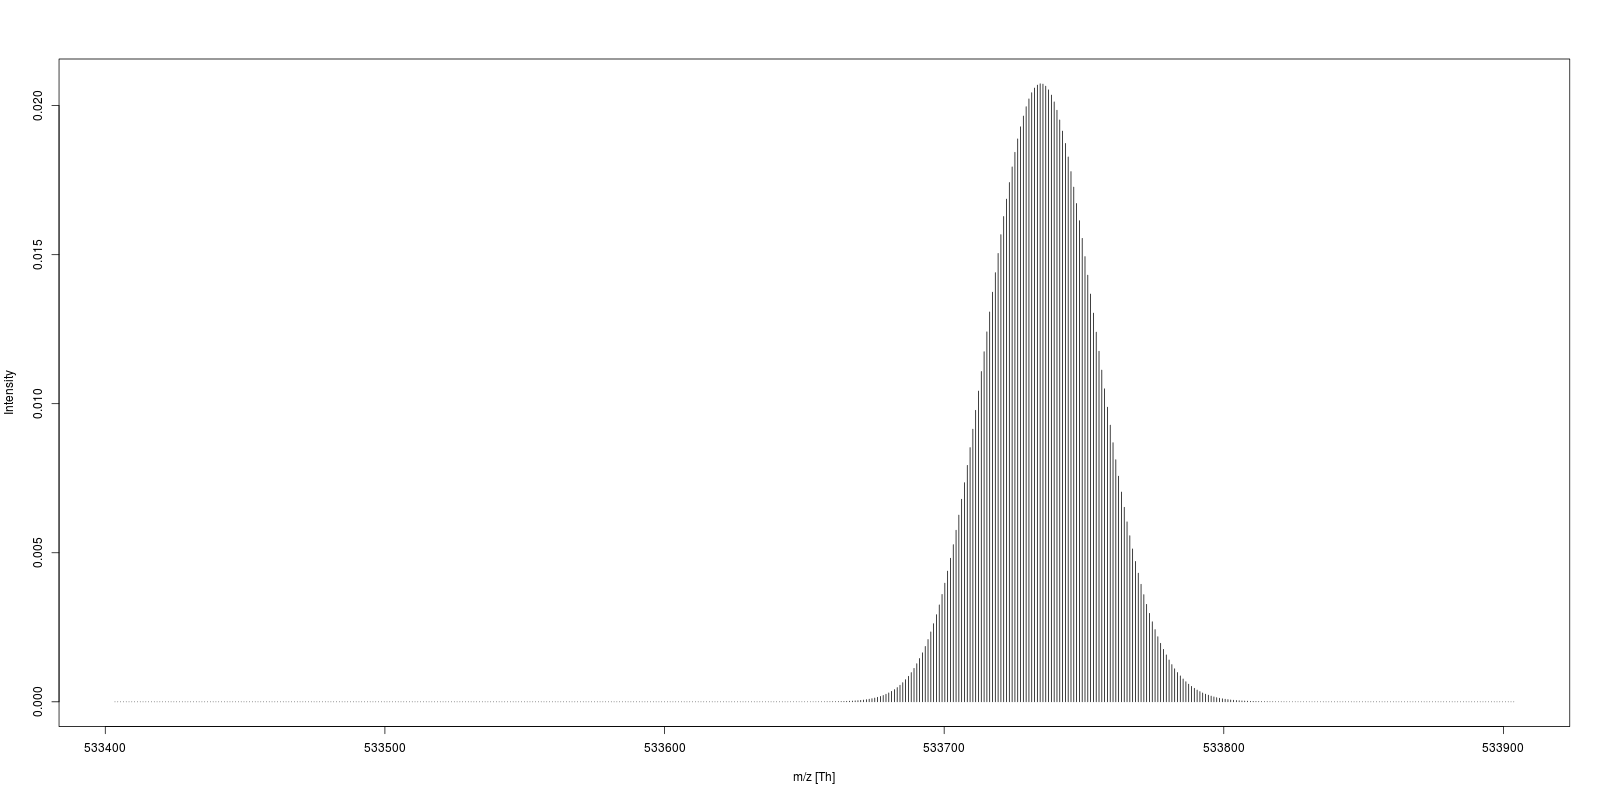
\includegraphics[width=.8\textwidth, keepaspectratio]{./picts/humanDynein.png}
		\end{center}
	\end{frame}

	%%%%%%%%%%%%%%%%%%%%%%%%%%%%%%%%%%%%%%%%%%%%%%%%%%%%%xetex%%%%%%%%%%%%%
	\begin{frame}\frametitle{Gaussian Approximation to Multinomial Model}

		\begin{itemize}
			\item Theoretical Spectra: $\Big\{ f_R(z) \Big\}_{R \in \text{Reactions}}$
			\item Empirical Spectrum: $y(z)$
			\item Linear model:
			$$ y(z) = \sum_{R} \alpha_R f_R (z) + \epsilon(z)$$
			\item Usual least squares humbug
			$$ ||\epsilon||^2 = \Big|\Big| y - \sum_{R} \alpha_R f_k \Big|\Big|^2 \rightarrow \min$$
			\begin{itemize}
				\item[s.t.] $\alpha_R \geq 0$
				\item[s.t.] $\sum_R \alpha_R \leq 1$
				\item[where] $ ||y||^2 = \sprod{y}{y} =  \int_\real y(x)^2 \mathrm{d}\,x.$ 
			\end{itemize}
		\end{itemize}
	\end{frame}

	%%%%%%%%%%%%%%%%%%%%%%%%%%%%%%%%%%%%%%%%%%%%%%%%%%%%%xetex%%%%%%%%%%%%%
	\begin{frame}\frametitle{Gaussian Approximation to Multinomial Model}

		$$ \Big|\Big| y - \sum_{R} \alpha_R f_k \Big|\Big|^2 = || y ||^2 - 2 \alpha^\tran \mathfrak{m} + \alpha^\tran \mathfrak{H} \alpha$$ 

		\begin{itemize}
			\item[where] $\mathfrak{m}^\tran = [ \dots, \sprod{y}{f_R}, \dots ]$
			\item[and] $\mathfrak{H} = [\sprod{f_R}{f_P}]_{R,P \in \text{Reactions}}$
			\item[] 			
			\item Easy to evaluate scalar product 
			$$ m(z) = \frac{1}{\sqrt{\pi \sigma^2}} e^{-\frac{(z-\mu)^2}{\sigma^2}}\text{ and } 
n(z) = \frac{1}{\sqrt{\pi \eta^2}} e^{\frac{(z-\eta)^2}{\nu^2}}
$$
			$$\sprod{m}{n} = \int_\real m(z)n(z) \mathrm{d}\,z  = \frac{1}{\sqrt{\pi (\sigma^2 + \nu^2)}}e^{-\frac{(\mu-\eta)^2}{\sigma^2+\nu^2}}$$  
			\item This problem is numerically very nice
			\begin{itemize}
				\item The Gramm Matrix is diagonally dominant, well conditioned. 
			\end{itemize}
		\end{itemize}

	\end{frame}

	\framedGraphic{Theoretically Explained Spectrum}{./picts/spectrum.png}
	%%%%%%%%%%%%%%%%%%%%%%%%%%%%%%%%%%%%%%%%%%%%%%%%%%%%%xetex%%%%%%%%%%%%%
\section[Plans]{What remains to be done?}

	\begin{frame}\frametitle{Whole lotta of things to do}
		\begin{itemize}
			\item Algorithmically 
			\begin{itemize}
				\item Optimise generation of Reactions: 
				\begin{itemize}
					\item $\heartsuit \diamondsuit = \diamondsuit \heartsuit$
				\end{itemize}
				\item Calibrate fitting procedures: 
				\begin{itemize}
					\item stick spectra more jazzy among chemists
					\item no-one uses gaussian approximations
				\end{itemize}
				\item Derive quick procedures for stick spectra generation: modify BRAIN.
			\end{itemize}
			\item Experimentally
			\begin{itemize}
				\item More substances to analyze
				\item Mixtures of substances 
			\end{itemize}
			\item Pragmatically
			\begin{itemize}
				\item What if the substance is not known?
			\end{itemize}
		\end{itemize}
	\end{frame}

	\begin{frame}\frametitle{massTodon potential}
		\begin{itemize}
			\item Understanding ETD statics
			\item Next step : understand dynamics
			\item Quantitative approach : potential characterisation of peptides through the use of MASS SPEC.
			\begin{itemize}
				\item But not certain yet how to do it yet
			\end{itemize}

		\end{itemize}
	\end{frame}

%%%%%%%%%%%%%%%%%%%%%%%%%%%%%%%%%%%%%%%%%%%%%%%%%%%%%%%%%%%%%%%%%%%%%%%%%%%%%%%%%%%%%%%%%%%%%%%%%%%%%%%%

	
	    
	\begin{thebibliography}{10}

		\beamertemplatebookbibitems
		
		\bibitem{computationalMethodsForMassSpec}
			Ingvar Eidhammer, Kristian Flikka, Lennart Martens, Svein-Ole Mikalsen,
			\emph{Computational Methods for Mass Spectrometry Proteomics}.
			Wiley-Interscience, 
			2007.
			
		\bibitem{computationalMethodsForMassSpec}
			Igor Kaltashov, Stephen J. Eyles
			\emph{Mass Spectrometry in Biophysics: Conformation and Dynamics of Biomolecules}.
			Wiley-Interscience, 
			2005.	
				
	\end{thebibliography}	

	% \begin{frame}[t]\frametitle{Bibliography}
	% 	\bibliographystyle{eccaNoNotes}
	% 	\bibliography{myBooks}
	% \end{frame}


	%%%%%%%%%%%%%%%%%%%%%%%%%%%%%%%%%%%%%%%%%%%%%%%%%%%%%%%%%%%%%%

\end{document}
  
  
%%%%%%%%%%%%%%%%%%%%%%%%%%%%%%%%%%%%%%%%%%%%%%%%%%%%%%%%%%%%%%%%%%%%%%%%%%%

